% woshiqiaoqiao

\documentclass{ctexbook}

% Bookmark

\usepackage{bookmark}

% Figure

\usepackage{amsmath, amssymb, pgfplots}
\pgfplotsset{compat = newest, width = 6cm}

% Caption

\usepackage[labelsep = space]{caption}
\renewcommand{\thefigure}{\thechapter.\arabic{figure}~}
\renewcommand{\thetable}{\thechapter.\arabic{table}~}
\DeclareCaptionFont{kaishu}{\kaishu}
\captionsetup{font = kaishu}

% Table 

\usepackage{multirow, float, booktabs, makecell}
\renewcommand{\arraystretch}{1.5}

% Font

\usepackage{textcomp, mathcomp, bm, circledtext}

% Structure

\usepackage{titlesec}
\let\oldchapter\chapter
\renewcommand\chapter{\clearpage\oldchapter}
\let\oldsection\section
\renewcommand\section{\clearpage\oldsection}
\let\oldsubsection\subsection
\renewcommand\subsection[1]{\oldsubsection{#1}\vspace{10pt}}

% Math

\everymath{\displaystyle}

\usepackage{graphicx}
\usepackage{ctex}
\xeCJKsetup{CJKmath = true}
\usepackage{amsmath}
\usepackage[top=2cm, bottom=2cm, left=3cm, right=3cm]{geometry}
\usepackage{setspace}
\usepackage{hyperref}
\usepackage{fancyhdr}
\usepackage{draftwatermark}
\SetWatermarkText{}
% \SetWatermarkLightness{0.95}
% \SetWatermarkScale{1}
\renewcommand{\headrulewidth}{0pt}
\fancyhf{}
\fancyhead{}
\fancyfoot[C]{\thepage}
\pagestyle{fancy}

% Custom

\newcommand\blue[1]{{\bf\color{blue}#1}}
\newcommand\red[1]{{\bf\color{red}#1}}
\newcommand\mathline[1]{\begin{equation}\color{red}\bm{#1}\end{equation}}
\newcommand\titlename[1]{\caption{#1}\label{#1}}

\title{\huge\textbf{中学物理}}
\author{田怿}
\date{\today}

\begin{document}

\maketitle
\thispagestyle{empty}

\ctexset{
	chapter={name={第,部分},number=\chinese{chapter}},
	section={number=\arabic{section}},
	subsection={number=\arabic{section}.\arabic{subsection}},
}
\tableofcontents
\setcounter{page}{0}
\thispagestyle{empty}

% \setstretch{1.05}

\part{热学}\thispagestyle{empty}

\Keyword{热学}{thermology},即研究物质热运动规律及其应用的物理学分支。

\chapter{热力学}

\Keyword{热力学}{thermodynamics},即从宏观角度研究物质的热运动性质及其规律的热学分支。

热力学的研究对象叫做\Keyword{热力学系统}{thermodynamic system},简称\blue{系统}。热力学系统是由大量分子组成的。

系统之外与系统发生相互作用的其他物体统称为\blue{外界}。

\section{分子动理论}

\subsection{分子动理论}
\Itemize{
\item \Keyword{分子动理论}{molecular kinetic theory},包括物质是由大量分子组成的,分子在\blue{永不停息}地做\blue{无规则}运动,分子之间存在相互作用力。
\item 分子直径约为 \blue{$\bf10^{-10}m$}。
\item 18g 水中含有水分子的个数约为 \blue{$\bf6.02\times10^{23}$},即为阿伏伽德罗常数 $N_{\text{A}}$。
\item 在研究物体的热运动性质和规律时,不必区分它们在化学变化中所起的不同作用,而把组成物体的微粒统称为\Keyword{分子}{molecule}。
\item 不同的物质在相互接触时\blue{自发地}彼此进入对方的现象叫做\Keyword{扩散}{diffusion}。
\item 扩散现象可以发生在气体、液体和固体之间。
\item 扩散现象是物质分子永不停息地做无规则运动的证据之一。
\item 悬浮微粒的无规则运动叫做\Keyword{布朗运动}{Brownian motion}。
\item \blue{悬浮微粒的无规则运动并不是分子的运动},但可以间接地反应液体分子运动的无规则性。
\item 分子的无规则运动叫做\Keyword{热运动}{thermal motion}。
\item \blue{温度}是\blue{分子热运动剧烈程度}的标志。
\item \blue{分子之间存在引力},\blue{分子之间存在斥力}。
\item 分子之间,引力和斥力\blue{同时存在}。
\item 分子间的作用力 $F$ 与分子间距离 $r$ 有关。即:
\newline 当 $r=r_0$ 时,分子间的作用力 $F$ 为 0,这个位置被称为\blue{平衡位置}。
\newline 当 $r>r_0$ 时,分子间的作用力 $F$ 表现为引力。
\newline 当 $r<r_0$ 时,分子间的作用力 $F$ 表现为斥力。
\begin{figure}[H]
	\centering
	\begin{tikzpicture}
	\begin{axis}[
		axis lines = middle,
		xmin = 0, xmax = 8,
		ymin = -4, ymax = 4,
		smooth, thick,
		xlabel = {$r$}, ylabel = {$F$},
		xlabel style = {anchor = north},
		ylabel style = {anchor = east},
		xtick = {0.83627}, xticklabels = {$r_0$}, 
		ytick = \empty,
		samples = 200,
		legend entries = {\kaishu{引力}, \kaishu{斥力}},
		legend style = {font = \small},
	]
		\addplot+[no marks, domain = 0.5 : 7.5]{6 / (x + 1) ^ 1.3};
		\addplot+[no marks, domain = 0.5 : 7.5]{-5 / (x + 1)};
	\end{axis}
	\node at (0, 2) [below = 5pt, left = -1pt] {$O$};
	\end{tikzpicture}
	~~
	\begin{tikzpicture}
	\begin{axis}[
		axis lines = middle,
		xmin = 0, xmax = 4,
		ymin = -2, ymax = 2,
		smooth, thick,
		xlabel = {$r$}, ylabel = {$F$},
		xlabel style = {anchor = north},
		ylabel style = {anchor = east},
		xtick = {0.46607}, xticklabels = {$r_0$}, xtick style = {anchor = north east},
		ytick = \empty,
		samples = 200,
		legend entries = {\kaishu{合力}},
		legend style = {font = \small},
	]
		\addplot+[no marks, domain = 0.25 : 3.75]{9 / ((x + 0.85) ^ 6) - 3 / ((x + 0.85) ^ 2)};
	\end{axis}
	\node at (0, 2) [below = 5pt, left = -1pt] {$O$};
	\end{tikzpicture}
	\Title{分子间的作用力与分子间的距离的关系}
\end{figure}
}

\subsection{固体~~液体~~气体}
\vspace{10pt}
\Itemize{
\item 固体分子间的距离小,不容易被压缩和拉伸,具有一定的体积和形状。
\item 气体分子间的距离很大,彼此间几乎没有作用力。具有流动性,容易被压缩。
\item 液体分子间的距离比气体小、比固体大,液体分子间的作用力比固体小、比气体大,分子没有固定的位置,运动较自由。液体较难被压缩,没有一定的形状,具有流动性。
\begin{table}[H]
	\kaishu
	\centering
	\begin{tabular}{ccccc}
	\toprule
	\multirow{2}*{物态} & \multicolumn{2}{c}{微观特性} & \multicolumn{2}{c}{宏观特性} \\
	& 分子间距离 & 分子间作用力 & 固定形状 & 固定体积 \\ 
	\midrule
	固态 & 很小 & 很大 & 是 & 是 \\ 
	液态 & 较大 & 较大 & 否 & 是 \\ 
	气态 & 很大 & 很小 & 否 & 否 \\ 
	\bottomrule
	\end{tabular}
	\Title{固体~~液体~~气体}
\end{table}
}
\section{内能}

\subsection{内能}
\Itemize{
\item 分子由于\blue{热运动}而具有的能量叫做\blue{分子动能}。
\item 系统中所有分子的动能的平均值叫做\blue{分子热运动的平均动能}。
\item 物体温度升高时,分子热运动的平均动能增加。
\item \blue{温度}是\blue{分子热运动的平均动能}的标志。
\item 单原子分子的平均动能 $\overline{E_k}=\frac32kT$,即 $\overline{E_k}\propto T$。其中 $k$ 是玻尔兹曼常数。
\item 分子之间由于存在\blue{相互作用力}而具有的能叫做\blue{分子势能}。
\item 分子势能 $E_p$ 与分子间的距离 $r$ 有关。即:
\newline 当 $r=r_0$ 时,分子间的作用力 $F$ 为 0,\blue{分子势能最小}。
\newline 当 $r>r_0$ 时,分子间的作用力 $F$ 表现为引力,分子势能减小。
\newline 当 $r<r_0$ 时,分子间的作用力 $F$ 表现为斥力,分子势能增大。
\item 分子势能的大小由\blue{分子间的相对位置}决定。如果选定分子间距离 $r$ 为无穷远时的分子势能 $E_p$ 为 0,则分子势能 $E_p$ 随分子间距离变化的情况如\FigureRef{分子势能与分子间的距离的关系}所示。
\begin{figure}[H]
	\centering
	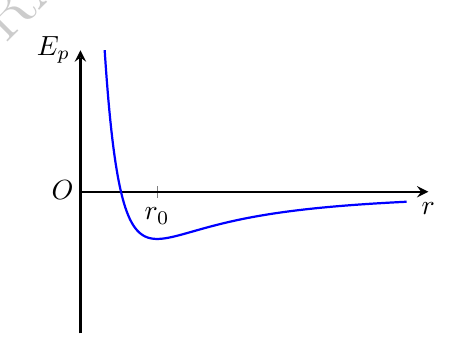
\begin{tikzpicture}
	\begin{axis}[
		axis lines = middle,
		xmin = 0, xmax = 4,
		ymin = -2, ymax = 2,
		smooth, thick,
		xlabel = {$r$}, ylabel = {$E_p$},
		xlabel style = {anchor = north},
		ylabel style = {anchor = east},
		xtick = {0.88205}, xticklabels = {$r_0$}, xtick style = {anchor = north east},
		ytick = \empty,
		samples = 200,
	]
		\addplot+[no marks, domain = 0.25 : 3.75]{9 / ((x + 0.85) ^ 6) - 3 / ((x + 0.85) ^ 2)};
	\end{axis}
	\node at (0, 2) [below = 5pt, left = -1pt] {$O$};
	\end{tikzpicture}
	\Title{分子势能与分子间的距离的关系}
\end{figure}
\item 分子势能与物体体积有关。
\item 物体中所有分子的\blue{分子动能与分子势能的总和},叫做物体的\Keyword{内能}{internal energy}。任何物体都具有内能。内能的单位是\blue{焦耳($\bf J$)}。
\item 物体的内能与\blue{温度}和\blue{体积}有关。
}

\subsection{比热容}
\Itemize{
\item 内能由\blue{高温}物体转移到\blue{低温}物体的过程叫做\blue{热传递}。
\item 热传递的基本方式包括传导、对流和辐射。
\item 在热传递过程中,传递能量的多少叫做\Keyword{热量}{quantity of heat}。用符号 \blue{$\bm Q$} 表示。单位是\blue{焦耳}。
\item 物体吸收热量是内能增加,放出热量时内能减少。\blue{热量是物体内能改变的量度}。
\item 一定质量的某种物体,在温度升高(或降低)时吸收(或放出)的热量与它的质量和升高(或降低)的温度乘积之比,叫做这种物质的\Keyword{比热容}{specific heat capacity}。用符号 \blue{$\bm c$} 表示。单位是\blue{焦每千克摄氏度($\bf J/(kg\cdot\textcelsius)$)}。有:
\Math{c=\frac{\Delta Q}{m\Delta t}}
\item 比热容是反映\blue{物质自身性质}的物理量。
\item 不同的物质,比热容一般不同。
\item 水的比热容为 \blue{$\bf4.2\times10^3J/(kg\cdot\textcelsius)$}。
\item 热量的计算有 \blue{$\bm{\Delta Q=cm\Delta t}$}。
\item \blue{热平衡方程},即 \blue{$\bm{\Delta Q_{\tiny\mbox{吸}}=\Delta Q_{\tiny\mbox{放}}}$}。
}
\section{热机}

\subsection{热机}
\Itemize{
\item \Keyword{热机}{heat engine},即利用内能做功(\blue{内能转化为机械能})的机械。
\item \blue{蒸汽机},即利用水蒸气膨胀做功的热机。蒸汽机属于外燃机。
\item 活塞从气缸的一端运动到另一端的过程叫做一个\blue{冲程}。
\item 四冲程汽油机一般包括\blue{吸气}、\blue{压缩}、\blue{做功}、\blue{排气}四个冲程。
\item \blue{汽油机}和\blue{柴油机}都属于\blue{内燃机}。
\item \blue{汽轮机}和\blue{喷气发动机}。
}

\subsection{热机的效率}
\Itemize{
\item 能够燃烧的物质叫做\blue{燃料}。
\item 在燃烧过程中,燃烧的\blue{化学能}转化为\blue{内能}。
\item 某种燃料\blue{完全燃烧}放出的能量与其质量或体积的比叫做这种燃料的\blue{热值}(combustion value)或燃烧值。用符号 \blue{$\bm q$} 表示。单位是\blue{焦耳每千克($\bf J/kg$)}或\blue{焦每立方米($\bf J/m^3$)}。有:
\Math{q=\frac{Q_{\tiny\mbox{放}}}m~~\mbox{或}~~q=\frac{Q_{\tiny\mbox{放}}}V}
\item 热值在数值上等于 \blue{$\bf1kg$} 或 \blue{$\bf1m^3$} 的某种燃料\blue{完全燃烧}放出的热量。其中 $1\text{m}^3$ 是\blue{标准状态}下气体燃料的体积。标准状态是指温度为 \blue{$\bf0\textcelsius$}、压强为 \blue{$\bf1\text{atm}$} 的状态。
\item 热量的计算有 \blue{$\bm{Q_{\tiny\mbox{放}}=qm}$} 或 \blue{$\bm{Q_{\tiny\mbox{放}}=qV}$}。
\item 做有用功的能量与燃料完全燃烧放出的能量之比叫做\blue{热机的效率},有:
\Math{\eta=\frac{Q_{\tiny\mbox{有用}}}{Q_{\tiny\mbox{燃料}}}\cdot100\%}
\item 设燃料放出的热量为 $Q_1$,热机吸收的热量为 $Q_2$,废气带走的热量为 $Q_3$,则:
$$
\eta=\frac{Q_1-Q_2-Q_3}{Q_1}\cdot100\%
$$
}
\section{热力学定律}

\subsection{系统内能的改变}
\Itemize{
\item 改变系统内能的两种方式是\blue{热传递}和\blue{做功}。
\item 在热传递过程中,系统吸收热量内能增加,放出热量内能减少。
\item 热量是\blue{热传递过程中}系统内能变化的量度。
\item 系统与外界没有热传递的过程叫做\Keyword{绝热过程}{adiabatic process}。
\item 在绝热过程中,外界对系统做功,系统内能增加;系统对外界做功,系统内能减少。
\item 做功是\blue{绝热过程中}系统内能变化的量度。
\item 焦耳的实验表明\blue{热传递和做功对改变系统的内能是等效的}。
}

\subsection{热力学第一定律}
\Itemize{
\item \Keyword{热力学第一定律}{first law of thermodynamics},即热力学系统内能 $U$ 的变化量等于系统从外界吸收的热量(系统向外界放出的热量)与外界对系统做的功(系统对外界做的功)之和。有:
\Math{\Delta U=Q+W}
系统对外界吸热,$Q$ 为正值;系统对外界放热,$Q$ 取负值;外界对系统做功,$W$ 取正值;系统对外界做功,$W$ 取负值。
}

\subsection{能量守恒定律}
\Itemize{
\item 不同形式的能量可以在一定条件下相互转化。
\item \Keyword{能量守恒定律}{law of conservation of energy},即能量既不会凭空产生,也不会凭空消失,它只能从一种形式\blue{转化}为其他形式,或者从一个物体\blue{转移}到其他物体,在转化或转移的过程中,能量的总量保持不变。
\item 能量守恒定律是自然界最普遍、最重要的基本定律之一。
\item 能量守恒定律的本质是\blue{时间平移对称性}。
\item \blue{永动机},即不需要动力就能源源不断地对外做功的机器,分为第一类永动机和第二类永动机。
\item 能量守恒定律的另一种表述为\blue{第一类永动机不可能制成}。
}

\subsection{热力学第二定律}
\Itemize{
\item 一切与热现象有关的宏观自然过程都是\blue{不可逆}的。
\item \Keyword{热力学第二定律}{second law of thermodynamics}。
\item \blue{克劳修斯表述},即热量不能\blue{自发}地从低温物体传到高温物体。自发是指不需要任何第三者的介入,不会对任何第三者产生任何影响。自发的方向是从高温物体指向低温物体。
\item 克劳修斯表述阐述了\blue{传热的方向性}。
\item \blue{开尔文表述},即\blue{不可能从单一热库吸收热量},使之完全变成功,而不产生其他影响。不可能从单一热库吸热,而且一定会向另一个热库放热。
\item 开尔文表述阐述了\blue{机械能与内能转化的方向性}。
\item \blue{热力学第二定理的另一种表述为}\blue{第二类永动机不可能制成}。
\item 热力学第二定律的克劳修斯表述和开尔文表述是\blue{等价的}。
\item \blue{能量耗散},即不同形式的能量最终都转化为\blue{内能}并分散在环境中的过程。
}

\chapter{统计物理}

\Keyword{统计物理}{statistical physics},即根据对物质微观结构及微观粒子相互作用的认识,用概率统计的方法,对由大量粒子组成的宏观物体的物理性质及宏观规律作出微观解释的热学分支。
\chapter{电磁学}

\newpage
{\bf 这里是一段关于电磁学的介绍.}

\newcommand\resistance{
	\begin{tikzpicture}[baseline = {([yshift = -3.5pt] current bounding box.center)}]
		\draw (0, 0) rectangle (0.6, 0.2);
		\draw (-0.3, 0.1) -- (0, 0.1);
		\draw (0.6, 0.1) -- (0.9, 0.1);
	\end{tikzpicture}
}

\newcommand\ammeter{
	
\begin{tikzpicture}[baseline = {([yshift = -3.5pt] current bounding box.center)}]
		\node (A) [circle, draw, scale = 1, inner sep = 1pt, line width = 0.5pt] at (0, 1){\small A};
	\end{tikzpicture}
} % ~{\Large\textcircled{\small A}}~

\newcommand\voltmeter{
	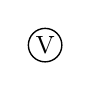
\begin{tikzpicture}[baseline = {([yshift = -3.5pt] current bounding box.center)}]
		\node (V) [circle, draw, scale = 1, inner sep = 1pt, line width = 0.5pt] at (0, 1){\small V};
	\end{tikzpicture}
} % ~{\Large\textcircled{\small V}}~

\newcommand\slidingrheostat{
	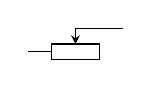
\begin{tikzpicture}[baseline = {([yshift = -3.5pt] current bounding box.center)}]
		\draw (0, 0) rectangle (0.6, 0.2);
		\draw (-0.3, 0.1) -- (0, 0.1);
		\draw [-stealth] (0.3, 0.4) -- (0.3, 0.2);
		\draw [line join = miter] (0.9, 0.4) -- (0.3, 0.4) -- (0.3, 0.3);
	\end{tikzpicture}
}

\section{电荷}

\vspace{10pt}
\begin{itemize}
\item 物体能够吸引轻小物体,就说物体带了电,即物体带了\blue{电荷}(electric charge)。带了电荷的物体叫做\blue{带电体}。
\item 使物体带电叫做\blue{起电}。用摩擦的方式使物体带电叫做\blue{摩擦起电}(electrification by friction)。
\item 自然界\blue{只有}两种电荷。
\item 用丝绸摩擦过的玻璃棒带的电荷叫做\blue{正电荷}(positive charge)。用毛皮摩擦过的橡胶棒带的电荷叫做\blue{负电荷}(negative charge)。
\item \blue{同种}电荷相互\blue{排斥},\blue{异种}电荷相互\blue{吸引}。
\item 电荷的多少叫做\blue{电荷量}(electric quantity),简称\blue{电量}。用 \blue{$\bm Q$} 或 \blue{$\bm q$} 表示。在国际单位制中,电荷量的单位是\blue{库仑}(coulomb),简称\blue{库}。符号是 \blue{$\bf C$}。正电荷的电荷量为正值,负电荷的电荷量为负值。
\item \blue{验电器}和\blue{静电计}。
\item 两种电荷互相完全抵消叫做\blue{中和}。
\item 物质是由\blue{分子}构成的,分子是由\blue{原子}构成的。
\item 原子是由带正电的\blue{原子核}和带负电的\blue{电子}(electron)组成的。
\item 原子核是由带正电的\blue{质子}和不带电的\blue{中子}组成的。
\item 每个原子中质子与电子的\blue{数量相等},质子与电子所带的\blue{电荷量相同}。
\item 摩擦起电的本质是电荷从一个物体\blue{转移}到另一个物体。
\item 金属原子中能脱离原子核的束缚而在金属中自由运动的电子叫做\blue{自由电子}(free electron)。
\item 失去自由电子的原子叫做\blue{离子}(ion)。
\item 质子、电子所带的电荷量(\blue{最小的电荷量})叫做\blue{元电荷}(elementary charge),用 \blue{$\bm e$} 表示。有:
\mathline{e\approx1.6\times10^{-19}\text{C}}
\item 所有带电体的电荷量都是 $e$ 的整数倍,不是连续变化的,即量子化的。
\item 电子的电荷量 $e$ 与质量 $m_e$ 之比叫做\blue{电子的比荷}(specific charge)。电子的质量 $m_e=9.11\times10^{-31}\text{kg}$,则电子的比荷为:
$$
\frac{e}{m_e}\approx1.76\times10^{11}\text{C}/\text{kg}
$$
\item 利用静电感应使金属带电叫做\blue{感应起电}(electrification by induction),所带电荷叫做\blue{感应电荷}(induced charge)。
\item \blue{静电感应}(electrostatic induction)。
\item 三种常见的起电方式包括摩擦、接触、感应。
\item \blue{电荷守恒定律}(law of conservation of charge),即电荷既不会创生,也不会消灭。它只能从一个物体转移到另一个物体,或者从物体的一部分转移到另一部分。在转移的过程中,电荷的总量保持不变。
\item 一个与外界没有电荷交换的系统,电荷的\blue{代数和}保持不变。
\item 电荷守恒定律是自然界最普遍、最重要的基本定律之一。
\end{itemize}
\section{电路}

\subsection{简单电路}
\Itemize{
\item \Keyword{电路}{electric circuit},即用导线将用电器、电源、开关连接起来。
\item \Keyword{电源}{power supply},即提供电能的装置,如电池、发电机。
\item \blue{用电器},即消耗电能的装置,如灯泡、电动机。
\item \blue{开关},即控制电路通断的装置,如单刀单掷开关、单刀双掷开关。
\item \blue{导线}通常由绝缘外皮和金属内芯(铜或铝)组成。
\item 处处连通的电路叫做\blue{通路}(\blue{闭合电路})。某处断开的电路叫做\blue{断路}(\blue{开路})。
\item \blue{直接}用导线将电源的正、负极连接起来的电路叫做\blue{短路}。
\item 闭合电路中,用电器两端被导线直接连通叫做用电器被\blue{短接}。
\item 用符号表示电路连接的图叫做\blue{电路图}。
\item \Keyword{串联}{series connection}和\Keyword{并联}{parallel connection}。
\item \blue{串联电路}和\blue{并联电路}。
\item 串联电路中各用电器相互影响,并联电路各用电器互不影响。
}

\subsection{电源}
\Itemize{
\item 能把电子从 A 搬运到 B 的装置 P 就是\Keyword{电源}{power source}。A 和 B 是电源的两个\blue{电极}。
}

\subsection{电流及其测量}
\Itemize{
\item 电荷的\blue{定向移动}形成电流。
\item 电路只有闭合时,电路中才有电流。
\item 规定\blue{正电荷}定向移动的方向为电流的方向。
\item 电子向某一方向定向移动等效于正电荷向相反方向定向移动。
\item 电路闭合时,\blue{电源外部}电流的方向是从电源正极经过用电器流向电源负极。
\item 电流强度是表示\blue{电流强弱程度}的物理量。
\item 单位时间内通过导体横截面的电荷量叫做\blue{电流强度},简称\Keyword{电流}{electric current}。用 \blue{$\bm I$} 表示。用 $q$ 表示在时间 $t$ 内通过导体横截面的电荷量,则有:
\Math{I=\frac qt}
\item 在国际单位制中,电流的单位是\Keyword{安培}{ampere},简称\blue{安}。符号是 \blue{$\bf A$}。\blue{$\bf 1A=1C/s$}。常用单位还有\blue{毫安}(\blue{$\bf mA$})和\blue{微安}(\blue{$\bf\textmu A$}),它们与安培的关系是 \blue{$\bf1mA=10^{-3}A$},\blue{$\bf1\textmu A=10^{-6}A$}。
\item 导体的横截面积为 $S$,\blue{自由电子数密度}(单位体积内的自由电子数)为 $n$,自由电子定向移动的平均速率为 $v$,电子的电荷量为 $e$,则:
$$
I=neSv
$$
\item 测量电路中电流大小的仪表叫做\blue{电流表},符号是\ammeter。
}

\subsection{电压及其测量}
\Itemize{
\item \Keyword{电压}{voltage}用 \blue{$\bm U$} 表示。单位是\Keyword{伏特}{volt},简称\blue{伏}。符号是 \blue{$\bf V$}。常用单位还有\blue{千伏}(\blue{$\bf kV$})和\blue{毫伏}(\blue{$\bf mV$}),它们与伏特的关系是 \blue{$\bf1kV=10^3V$},\blue{$\bf1mV=10^{-3}V$},\blue{$\bf1\textmu V=10^{-6}V$}。
\item 干电池的电压为 1.5V,铅蓄电池的电压为 2V。
\item 测量电路中两点间电压大小的仪表叫做\blue{电压表},符号是\voltmeter。
}

\subsection{串、并联电路中电流、电压的规律}
\Itemize{
\item 在串联电路中,电流处处相等。在并联电路中,干路电流等于各支路电流之和。
\item 在串联电路中,总电压等于各用电器两端电压之和。在并联电路中,各支路两端电压相等,等于总电压。
\item 串联电池组两端电压等于每节电池两端电压之和。并联电池组两端电压等于每节电池两端电压。
}

\subsection{电阻}
\Itemize{
\item 容易导电的物体叫做\Keyword{导体}{conductor}。不容易导电的物体叫做\Keyword{绝缘体}{insulator}。
\item 导电性能介于导体和绝缘体之间的物体叫做\Keyword{半导体}{semiconductor}。
\item 导体中有大量的能够自由移动的电荷(\blue{自由电荷}),而绝缘体很少。
\item 在外界\blue{温度}、\blue{压力}、\blue{光照}等条件发生改变或掺入杂质时,绝缘体有可能变成导体。
\item \Keyword{电阻}{resistance}是表示导体对电流阻碍作用大小的物理量,用 \blue{$\bm R$} 表示。单位是\blue{欧姆},简称\blue{欧},符号是 \blue{$\bm\Omega$}。常用单位还有千欧(\blue{${\bf k}\bm\Omega$})、兆欧(\blue{${\bf M}\bm\Omega$}),换算关系为 \blue{$\bf1k\bm\Omega=10^3\bm\Omega$},\blue{$\bf1M\bm\Omega=10^6\bm\Omega$}。
\item 具有一定电阻值的元件叫做\blue{电阻器},也叫做\blue{定值电阻},简称\blue{电阻},符号是\resistance。
\item \blue{电流表的电阻很小},\blue{电压表的电阻很大}。
\item 导体的电阻与导体的材料、长度、横截面积和温度有关。
\item \blue{$\bm{R=\dfrac UI}$}。
\item \blue{电阻定律},即同种材料的导体,其电阻 \blue{$\bm R$} 与它的长度 \blue{$\bm l$} 成正比,与它的横截面积 \blue{$\bm S$} 成反比。导体电阻还与\blue{材料}有关。有:
\Math{R=\rho\frac lS}
\blue{$\bm\rho$} 叫做材料的\Keyword{电阻率}{resistivity}。
\item \blue{金属的电阻率随温度的升高而增大}。
\item 当温度降低到某一温度时,物质的\blue{电阻变为零},这种现象叫做\blue{超导现象}。发生超导现象的物质叫做\Keyword{超导体}{superconductor},物质出现超导现象的温度叫做\blue{临界温度}或\blue{转变温度}。
\item 用横坐标表示电压 $U$,纵坐标表示电流 $I$。画出的 $I-U$ 图像叫做导体的\blue{伏安特性曲线}。
\item 电流与电压成正比的电学元件叫做\blue{线性元件}。电流与电压不成正比的电学元件叫做\blue{非线性元件}。
\item 能改变接入电路中电阻大小的元件叫做\blue{变阻器}。其作用包括保护电路、改变电流、控制电压。
\item \blue{滑动变阻器}的符号是\slidingrheostat。
}
\section{欧姆定律}

\subsection{电流与电压、电阻的关系}
\Itemize{
\item 在\blue{电阻一定}时,通过导体的电流与导体两端的电压成正比。
\item 在\blue{电压一定}时,通过导体的电流与导体的电阻成正比。
\item \Keyword{欧姆定律}{Ohm's law},即导体中的电流,跟导体两端的电压成正比,跟导体的电阻成反比。有:
\Math{I=\frac UR}
欧姆定律对金属、电解液适用,对半导体、电离气体不适用。
}

\subsection{电阻的测量}
\Itemize{
\item 伏安法测电阻,即利用 $R=\frac UI$ 测量电阻。
\item 小灯泡是非线性元件,其伏安特性曲线如\FigureRef{小灯泡的伏安特性曲线}所示。
\begin{figure}[H]
	\centering
	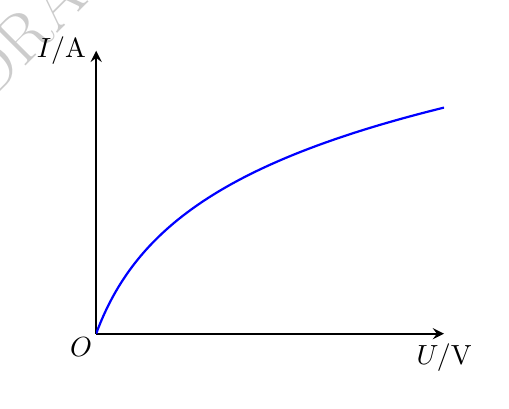
\begin{tikzpicture}
	\begin{axis}[
		axis lines = middle,
		xmin = 0, xmax = 10,
		ymin = 0, ymax = 10,
		smooth, thick,
		xlabel = {$U/\text{V}$}, ylabel = {$I/\text{A}$},
		xlabel style = {anchor = north},
		ylabel style = {anchor = east},
		xtick = \empty,	ytick = \empty,
		samples = 200,
	]
		\addplot+[no marks, domain = 0 : 10]{log10(x + 1) / log10(1.35)};
	\end{axis}
	\node at (0, 0) [below = 5pt, left = -2pt] {$O$};
	\end{tikzpicture}
	\Title{小灯泡的伏安特性曲线}
\end{figure}
}

\subsection{串、并联电路中的分压、分流规律}
\Itemize{
\item 串联分压,即 \blue{$\bm{U_1:U_2:\cdots:U_n=R_1:R_2:\cdots:R_n}$}。
\item 并联分流,即 \blue{$\bm{I_1:I_2:\cdots:I_n=\frac1{R_1}:\frac1{R_2}:\cdots:\frac1{R_n}}$}。
}

\subsection{串、并联电路中电阻的关系}
\Itemize{
\item 若电阻 $R$ 产生的效果与两个电阻 $R_1$ 和 $R_2$ 产生的效果相同,则电阻 $R$ 叫做 $R_1$ 和 $R_2$ 的\blue{等效电阻}。
\item 在串联电路中,有 \blue{$\bm{R=R_1+R_2+\cdots+R_n}$},即\blue{串联电路中,等效电阻等于各串联电阻之和}。
\item 在并联电路中,有 \blue{$\bm{\frac1R=\frac1{R_1}+\frac1{R_2}+\cdots+\frac1{R_n}}$},即\blue{并联电路中,等效电阻的倒数等于各并联电阻的倒数之和}。
\item 两个电阻 $R_1$ 和 $R_2$ 并联时,其等效电阻 \blue{$\bm{R=\frac{R_1R_2}{R_1+R_2}}$}。
}
\section{电功和电功率}

\subsection{电功和电能}
\Itemize{
\item \Keyword{电能}{electric energy}可以转化为其他形式的能。单位是\blue{焦耳},简称\blue{焦},符号是 \blue{$\bf J$}。常用单位还有\blue{千瓦时},简称\blue{度},符号是 \blue{$\bf kW\cdot h$}。换算关系是 \blue{$\bf 1kW\cdot h=3。6\times10^6J$}。
\item 电流做的功叫做\Keyword{电功}{electric work}。用 \blue{$\bm W$} 表示。单位是\blue{焦耳},简称\blue{焦},符号是 \blue{$\bf J$}。
\item 电流做了多少功,就有多少电能转化为其他形式的能。
\item 电功等于电压 $U$、电流 $I$ 和通电时间 $t$ 的乘积,即:
\Math{W=UIt}
\item 根据 $U=IR$,电流通过电阻 $R$ 做的功为:
$$
W=I^2Rt~~或~~W=\frac{U^2}Rt
$$
\item 电功或电能的计量仪器叫做\blue{电能表}(电度表)。
}

\subsection{电功率}
\Itemize{
\item \Keyword{电功率}{electric power}是表示\blue{电流做功快慢}的物理量。用 \blue{$\bm P$} 表示。单位是\blue{瓦特},简称\blue{瓦},符号是 \blue{$\bf W$}。常用单位还有千瓦(\blue{$\bf kW$})、毫瓦(\blue{$\bf mW$})。换算关系是 \blue{$\bf1kW=10^3W$},\blue{$\bf1mW=10^{-3}W$}。
\item 电功率等于电流 $U$ 和电压 $I$ 的乘积,即:
\Math{P=\frac Wt=UI}
\item 根据 $U=IR$,电流通过电阻 $R$ 的电功率为:
$$
P=I^2R~~或~~P=\frac{U^2}R
$$
\item 用电器正常工作时的电压叫做\Keyword{额定电压}{rated voltage},用电器在额定电压下工作时的电功率叫做\Keyword{额定功率}{rated power}。
}

\subsection{焦耳定律}
\Itemize{
\item 电流通过导体的电能转化为内能,这种现象叫做\blue{电流的热效应}。
\item 电流的效应包括热效应、磁效应和化学效应。
\item \Keyword{焦耳定律}{Joule's law},即电流通过导体产生的热量 $Q$ 跟电流 $I$ 的二次方成正比,跟导体的电阻 $R$ 成正比,跟通电时间 $t$ 成正比。即:
\Math{Q=I^2Rt}
}
\section{磁}

\subsection{磁现象}
\begin{itemize}
\item 能够吸引\blue{铁}、\blue{钴}、\blue{镍}等物质的性质叫做\blue{磁性}(magnestion)。
\item 具有磁性的物体叫做\blue{磁体}(magnet)。
\item 磁性最强的两个部位叫做\blue{磁极}(magnetic pole)。
\item 能够自由转动的磁体,静止时由指向北方的磁极叫做\blue{北极}(north pole)或 \blue{N 极},指向南方的磁极叫做\blue{南极}(south pole)或 \blue{S 极}。
\item 磁极间相互作用的规律,即\blue{同名磁极相互排斥},\blue{异名磁极相互吸引}。
\item 原本没有磁性的物体在磁体或电流的作用下获得磁性的过程叫做\blue{磁化}(magnestization)。
\item 能够被磁化的物质统称为\blue{磁性材料}。
\item 磁性材料分为硬磁性材料和软磁性材料。
\item 被磁化后能够长期保持磁性的材料叫做\blue{硬磁性材料}(永磁体)。被磁化后不能长期保持磁性的材料叫做\blue{软磁性材料}。
\end{itemize}

\subsection{磁场(magnestion field)}
\begin{itemize}
\item \blue{磁场}的\blue{基本性质},即磁场对放入其中的磁体有力的作用。
\item 磁场中的不同位置磁场的强弱和方向不同。
\item \blue{规定}小磁针静止时 \blue{N 极所指的方向}为这点磁场的方向。
\item \blue{磁感线}(magnetic induction line)\blue{不存在},只是为了方便形象地描述磁场。
\item 磁体外部的磁感线都是从磁体的 \blue{N 极出发回到 S 极}。
\item \blue{磁感线疏密表示磁场强弱}。磁感线稀疏的地方磁场弱,磁感线密集的地方磁场强。
\item 磁感线上某点的\blue{切线方向},既是放在该处的小磁针 \blue{N 极的受力方向},也是该点的\blue{磁场方向}。
\item 地球周围空间存在的磁场叫做\blue{地磁场}。
\item 地磁的 N 极在地理的南极附近,地磁的 S 极在地理的北极附近。
\item 地磁场的两级和地理的两级不重合。
\item 地磁场的磁感线分布跟条形磁体的磁场相似。
\item 磁针所指南北方向偏离地理南北方向的角度叫做\blue{磁偏角}。
\end{itemize}

\subsection{电流的磁感应}
\begin{itemize}
\item 奥斯特实验。
\item 通电导线周围存在与电流方向有关的磁场,这种现象叫做\blue{电流的磁效应}。
\item 通电\blue{螺线圈}(\blue{线圈})外部的磁场与条形磁体的磁场相似。
\item \blue{安培定则}(Anpere's rule)或\blue{右手螺旋定则}(right-handed screw rule)。
\end{itemize}

\subsection{电磁铁及其应用}
\begin{itemize}
\item \blue{电磁铁}(electromagnet),即\blue{线圈}与\blue{铁芯}的组合。
\item 有电流时产生磁性,没有电流时失去磁性。
\item 匝数一定时,\blue{电流}越大,电磁铁的磁性越强。电流一定时,\blue{匝数}越多,电磁铁的磁性越强。
\item \blue{继电器}是利用低电压、弱电流电路的通断,来间接地控制高电压、强电流电路通断的装置。
\item \blue{电磁继电器}是利用电磁铁来控制工作电路的一种开关。其工作电路由\blue{低压控制电路}和\blue{高压工作电路}两部分构成。
\end{itemize}

\subsection{安培力与电动机}
\begin{itemize}
\item 通电导线在磁场中受到力的作用,力的方向跟电流的方向、磁场的方向有关,这个力叫做\blue{安培力}。
\item \blue{左手定则}(left-hand rule)。
\item 电动机是将电能转化为其他形式能的装置。
\item 电动机分为\blue{直流电动机}和\blue{交流电动机}。
\item 电动机由转子和定子两部分组成。能够转到的部分(线圈)叫做\blue{转子},固定不动的部分(磁体)叫做\blue{定子}。
\end{itemize}

\subsection{电磁感应与发电机}
\begin{itemize}
\item \blue{闭合电路}的\blue{一部分导体}在磁场中做\blue{切割磁感线}运动时,导体中就产生电流,这种现象叫做\blue{电磁感应}(electromagnetic induction)。产生的电流叫做\blue{感应电流}(induction current)。
\item \blue{右手定则}(right hand rule)。
\item 发电机是将其他形式能转化为电能的装置。
\item 发电机分为\blue{直流发电机}和\blue{交流发电机}。
\item 发电机由\blue{转子}(转动部分)和\blue{定子}(固定部分)两部分组成。
\item 方向随时间变化的电流叫做\blue{交变电流}(alternating current),简称\blue{交流},符号 \blue{AC}。方向不随时间变化的电流叫做\blue{直流电流}(direct current),简称\blue{直流},符号 \blue{DC}。
\item 交变电流的频率在数值上等于电流在每秒内周期性变化的次数。
\item 我国电网以交流供电,频率为 \blue{50Hz}。
\end{itemize}

\end{document}
